\documentclass[a4paper]{article}
\usepackage{amsfonts}
\usepackage{amsmath}
\usepackage{amssymb}
\usepackage{graphicx}  
\usepackage{cancel}

\newcommand{\degree}{^{\circ}}
\newcommand{\cis}{\operatorname{cis}}
\newcommand{\Bgsin}{\operatorname{Bgsin}}
\newcommand{\Bgcos}{\operatorname{Bgcos}}
\newcommand{\Bgtan}{\operatorname{Bgtan}}
\newcommand{\limit}{\lim\limits}
\newcommand{\summation}{\displaystyle\sum}
\newcommand{\dom}{\operatorname{dom}}

\begin{document}
  
\noindent \large Auteur: Rune Suy \\
\noindent \large Studierichting: Informatica\\
\noindent \large Oefeningenreeks 3G nr. 11.4\\

\medskip

\normalsize

$f(x) = \dfrac{3x^2 - 12x + 9}{x-2}$\\

1. Domein van $f(x)$:\\

$\dom(f) = \mathbb{R}\backslash\{2\}$\\

2. Asymptoten:\\

$\limit_{x \rightarrow 2 -} f(x) = \limit_{x \rightarrow 2 -} \dfrac{-3}{0} = +\infty$\\

$\limit_{x \rightarrow 2 +} f(x) = \limit_{x \rightarrow 2 -} \dfrac{-3}{0} = -\infty$\\

Er is dus een verticale asymptoot in $x = 2$. Langs links gaat $f$ naar $+\infty$, \\

langs rechts naar $-\infty$\\

$\limit_{x \rightarrow \infty} \dfrac{f(x)}{x} = \limit_{x\rightarrow\infty} \dfrac{3x^2 + 12x + 9}{x^2 - 2x} = 3 = a$\\

$\limit_{x \rightarrow \infty} f(x) - ax = \limit_{x\rightarrow \infty} \dfrac{\cancel{3x^2} - 12x + 9 - \cancel{3x^2} + 6x}{x-2} = \limit_{x\rightarrow \infty} \dfrac{-6x}{x} = -6$\\

SA: $y=3x-6$\\

geen HA\\

$f(x) - 3x + 6 = \dfrac{\cancel{3x^2} - \cancel{12x} + 9 - \cancel{3x^2} + \cancel{6x} + \cancel{6x} - 12}{x-2} = \dfrac{-3}{x-2}$\\

TO:\\

\begin{tabular}{c | c c c}
    $x$             &       & $2$   & \\ \hline
    $T$             & $-$   & $-$   & $-$ \\
    $N$             & $-$   & $0$   & $+$ \\ \hline
    $f(x) - 3x + 6$ & $+$   & $|$   & $-$ \\
\end{tabular}

\medskip

dus $f$ ligt boven SA bij $-\infty$ en onder SA bij $+\infty$\\

3. Tekenonderzoek van $f(x)$:\\

$D = 144 - 4 \cdot 3 \cdot 9 = 36$\\

$x_1 = \dfrac{12 + 6}{6} = 3$\\

$x_2 = \dfrac{12 - 6}{6} = 1$\\

TO:\\

\begin{tabular}{c | c c c c c c c}
    $x$             &       & $1$   &       & $2$   &       & $3$   & \\ \hline
    $T$             & $+$   & $0$   & $-$   & $-$   & $-$   & $0$   & $+$ \\
    $N$             & $-$   & $-$   & $-$   & $0$   & $+$   & $+$   & $+$ \\ \hline
    $f(x) - 3x + 6$ & $-$   & $0$   & $+$   & $|$   & $-$   & $0$   & $+$\\
\end{tabular}

\bigskip

4. Tekenonderzoek $f'(x)$:\\

$f'(x) = d \left( \dfrac{3x^2 - 12x + 9}{x - 2} \right) = \dfrac{(6x-12)(x-2) - (3x^2 - 12x + 9)}{(x-2)^2}$\\

$ = \dfrac{6x^2 - 12x - 12x + 24 - 3x^2 + 12 - 9}{(x-2)^2} = \dfrac{3x^2 - 12x + 15}{(x-2)^2}$\\

T:
$D = 144 - 4 \cdot 3 \cdot 15 = -36$\\

\begin{tabular}{c | c c c}
    $x$     &       & $2$   & \\ \hline
    $T$     & $-$   & $-$   & $-$ \\
    $N$     & $-$   & $0$   & $+$ \\ \hline
    $f'(x)$ & $+$   & $|^{(2)}$   & $-$ \\ \hline
    $f(x)$  & $\nearrow$ & $|$   & $\nearrow$\\
\end{tabular}

\bigskip

5. Tekenonderzoek $f''(x)$:\\

$f''(x) = d\left(\dfrac{3x^2-12x+15}{(x-2)^2}\right) = \dfrac{(6x-12)(x^2-4x +4) - (2x-4)(3x^2-12+15)}{(x-2)^4} $\\

$ = \dfrac{-6x+12}{(x-2)^4} = \dfrac{-6(x-2)}{(x-2)^4} = \dfrac{-6}{(x-2)^3}$\\

TO:\\

\begin{tabular}{c | c c c}
    $x$      &       & $2$      & \\ \hline
    $T$      & $-$   & $-$      & $-$ \\
    $N$      & $-$   & $0$      & $+$ \\ \hline
    $f''(x)$ & $+$   & $|^{(3)}$   & $-$ \\ \hline
    $f(x)$  & $\smile$ & $|$   & $\frown$\\
\end{tabular}

\newpage

\bigskip

6. Schets:\\

\begin{figure}[h]
    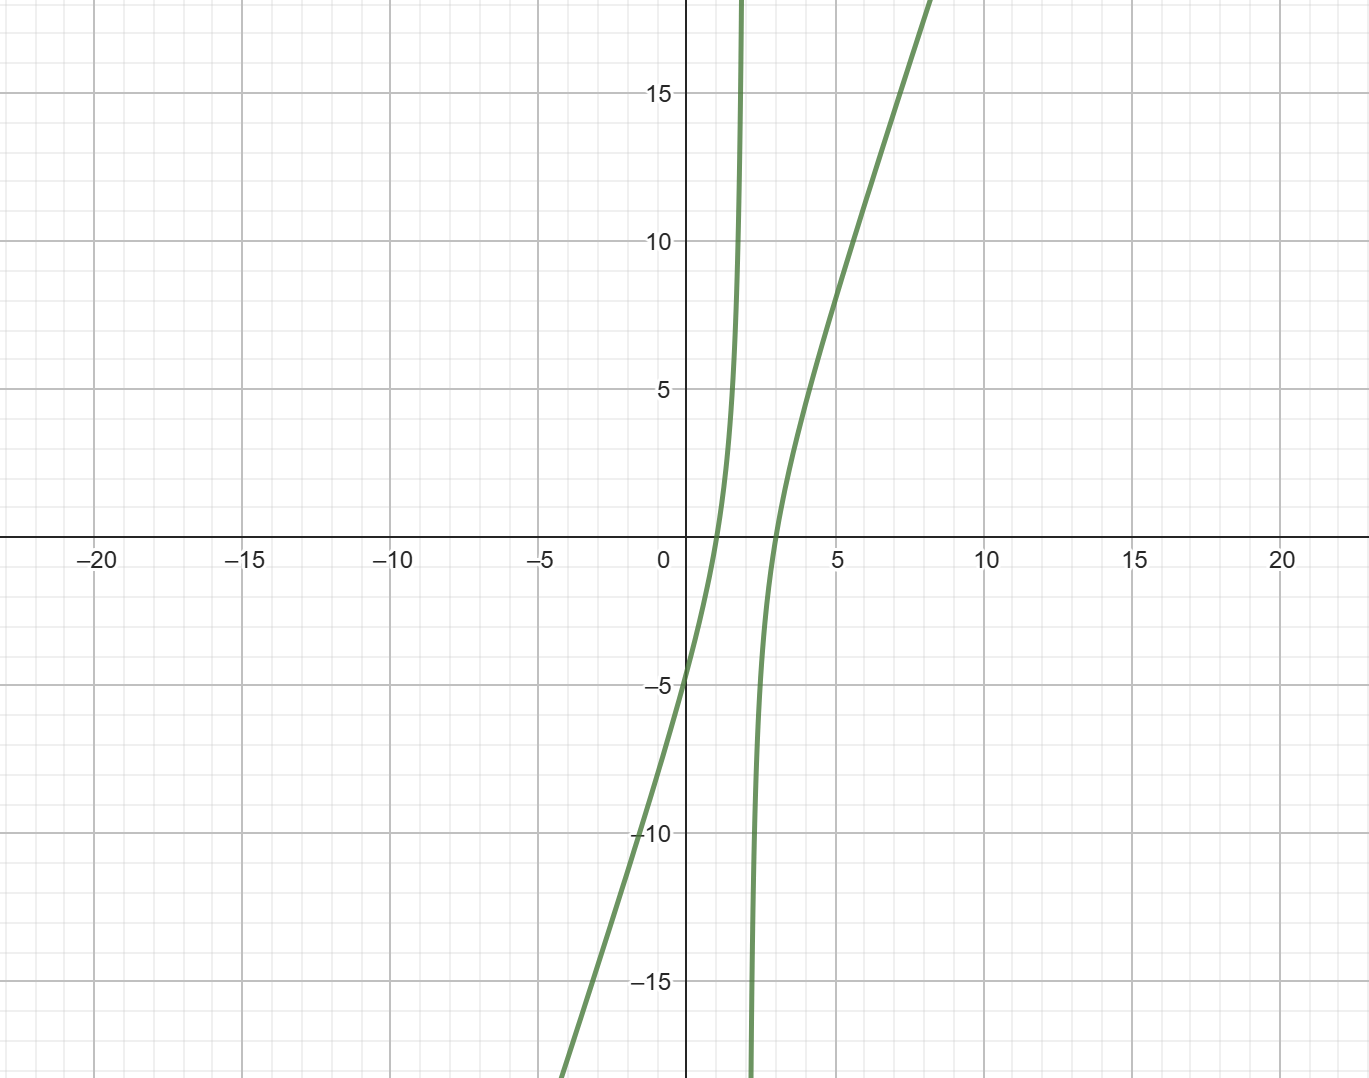
\includegraphics[width=\linewidth]{3G-11.4-rune.suy.INF.png}\\
\end{figure}
\begin{thebibliography}{999}
%\bibitem{a} Referentie
\end{thebibliography}
\end{document} 
